\subsubsection{Exercise}

Using simulink we simulate the closed-loop system for an input:
$$ r(t) = \left\{\begin{array}{rcl} r_1(t) & = & u_{t\geq 100} \\ r_2(t) & = & u_{t\geq 500} \end{array}\right.$$

\paragraph{Minimum phase model}

Figure \ref{simum} shows the output $y_1$ and $y_2$ of the closed-loop system in the minimum phase case. 
The control quality is the following: 
\begin{center}
\begin{tabular}{|c|ccc|}
    \hline
    & Overshoot& Overshoot& Rise\\ 
    & coupled & non-coupled & time \\
    \hline
    $y_1$ & $12\%$ & $0.1$ & $30$s  \\
    $y_2$ & $13\%$ & $0.1$ & $30$s  \\
    \hline
\end{tabular}
\end{center}

\begin{figure}[h!t]
    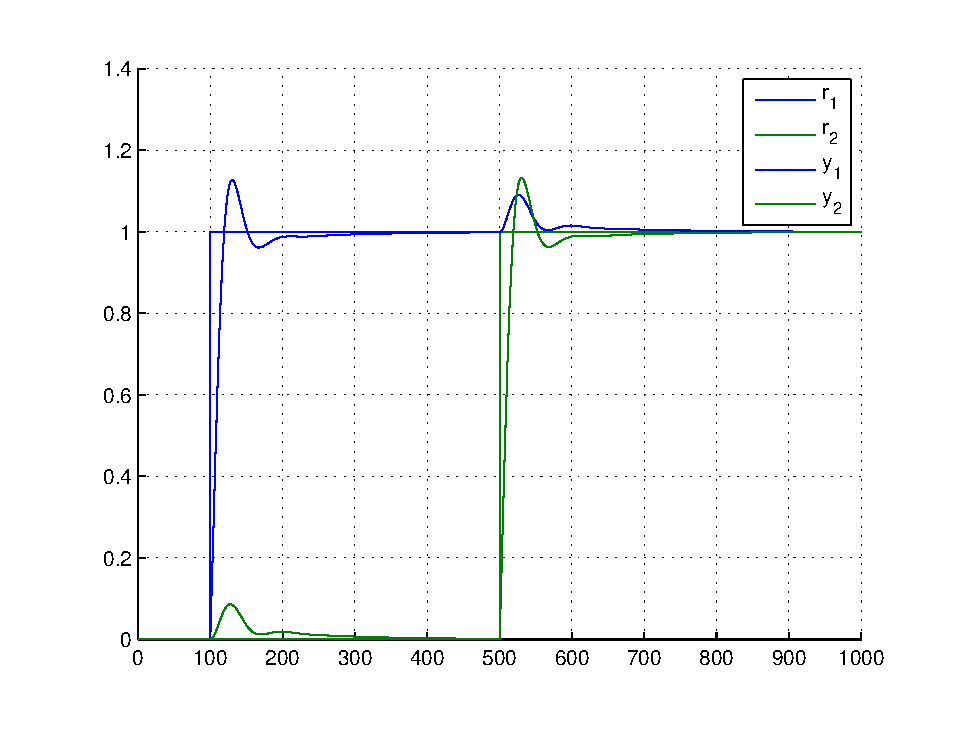
\includegraphics[width=\columnwidth]{fig/controlledouputm.eps}
    \caption{Response of the minimum phase system to $r(t)$}
    \label{simum}
\end{figure}

\paragraph{Non-minimum phase model}

Figure \ref{simunm} shows the output $y_1$ and $y_2$ of the closed-loop system in the non-minimum phase case. 
The control quality is the following: 
\begin{center}
\begin{tabular}{|c|ccc|}
    \hline
    & Overshoot& Overshoot& Rise\\ 
    & coupled & non-coupled & time \\
    \hline
    $y_1$ & $0\%$ & $0.5$ & $350$s  \\
    $y_2$ & $0\%$ & $0.35$ & $200$s  \\
    \hline
\end{tabular}
\end{center}

\begin{figure}[h!t]
    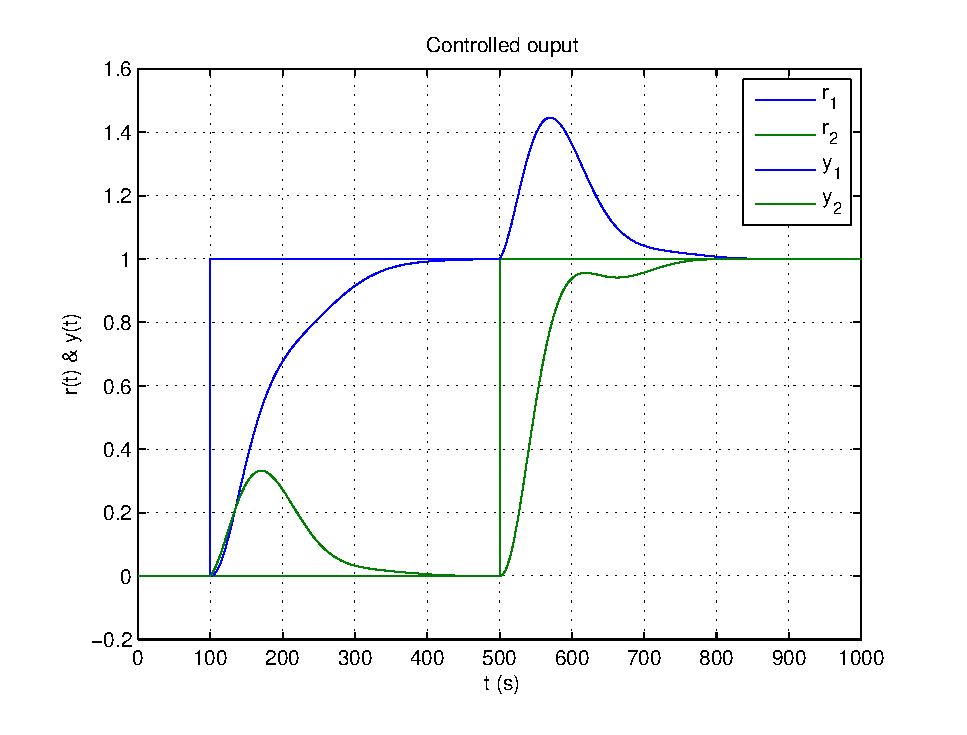
\includegraphics[width=\columnwidth]{fig/controlledouputnm.eps}
    \caption{Response of the non-minimum phase system to $r(t)$}
    \label{simunm}
\end{figure}

\paragraph{Results}

Figure \ref{simum} \& \ref{simunm} shows that the outputs are indeed coupled. 
However the control performance are more satisfying in the minimum-phase case. This is legit since the minimum-phase system do not present a RHP zero.
